This section describes the basic concept of the \textit{Smart Shelf}. 
The basic idea of the Smart Shelf is to enhance the interaction with shelves to work with these more effective and to improve the interaction. 
To satisfy these objectives some core features are proposed in this section. 
Figure \ref{fig:example_shelf} shows a similar shelf used for the project prototype which is small but satisfies the requirements for this prototype. 
However, one important fact which should be considered is the scalability. 
The applied techniques should be feasible in a technical and economical way. 
%
\begin{figure}
	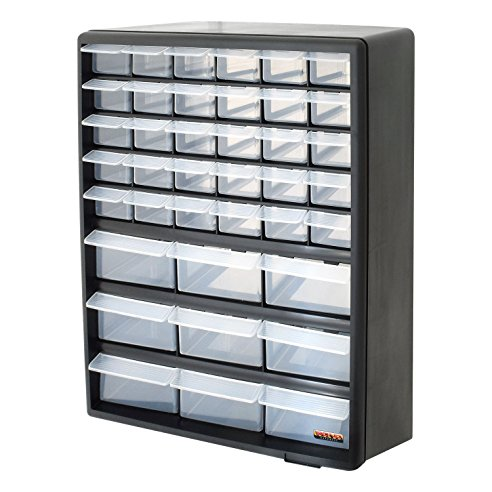
\includegraphics[width=0.9\columnwidth]{figures/example-prototype-shelf}
	\caption{Example for used Shelf as prototype}~\label{fig:example_shelf}
\end{figure}
%
\\
\\
The first problem the Smart Shelf wants to address is the fact that it is hard to find a specific item in a high amount of drawers. 
To do this we propose visual feedbacks combined with an user interface to submit search queries. 
The user interface can be used to insert a search word, for example the name of the searched item. 
This search query results in a visual feedback on the Smart Shelf, or in detail on the specific drawer where the item is contained. 

The user interface will be provided as webapp. 
The platform independence of a webapp leads to this design decision. 
In a first iteration mobile apps are considered, but were discarded because of the platform dependency (Android, Apple iOS, Microsoft Windows, etc.). 
Additionally, more features are provided by the webapp. 
Overall, it provides all functionalities to interact with the Smart Shelf. 
The search, control the shelf or getting more data about different items. 
For getting more information about a specific item the user interface provides additionally to a datasheet-like page the capability to scan QR-Codes. 
These QR-Codes are mounted on each drawer and encode the id of the drawer. 
A central server, which also serves the webapp holds the state of the Smart Shelf and has a mapping of these scanned ids to drawers and items. 
The different items contained in the shelf, the amount of them and current searches are called here as \textit{state}. 

As mentioned before an unsatisfying fact is, if the user search for a while for a specific item and finally find it, the drawer is empty. 
To address this problem the Smart Shelf provides a \textit{predictive management system} (abbr. PMS). 
This PMS enables the system to send notifications to operators if a drawer is empty or almost empty. 
Notifications enables the operators to react early to items with low or zero amount. 
This decreases the chance of out of stock items. 
To realize such a PMS data are needed for analysis and reaction based on specific conditions. 
Every drawer will get a electronic unit to measure the weights of the items in a drawer. 
Theses measurements are send to the server, which calculates with the stored weight of the specific item, the amount of items in that drawer. 
This enables the PMS to have an overview of the state about all items contained in drawers. 
Additionally to notifications a visual feedback is given at the shelf itself. 
Empty drawers are marked with a red light to indicate this to users directly. 

As mentioned before visual feedback is a central point in the design of the Smart Shelf. 
Therefore, it is used to indicate the searched drawer to the user and if a drawer is empty. 
However, the prototype uses visual feedback additionally for a so called \textit{service mode}, which can be switched on and off.
During service mode every drawer visualizes its state with different colours. 
Blue colour, if the drawer contains more items than a specified threshold. 
Yellow colour as warning, if there are less items than the threshold and a red colour, if there are zero items left. 
For this service mode the data acquired with the weight measurement are consulted. 

\subsection{Visual Feedback Colours}


\subsection{Assumptions}
To realize this prototype some preconditions are assumed which are listed in this section. 
\\
\\
All items in the shelf are either without packaging or with packaging. 
There will be no drawer where items are mixed. 
Furthermore, at any time there is only one sort of items in one drawer. 
Every drawer contains different items. 
The weight of a specific item is stored in the server for the amount calculation. 